\documentclass[]{beamer}

%%%%%%%%%%%%%%%%%%%%%%%%%%%%%%%%%%%%%%%%%%%%%%%%%%%%%%%%%%
% Slides pour la présentation de Rathaxes interne au LSE %
%%%%%%%%%%%%%%%%%%%%%%%%%%%%%%%%%%%%%%%%%%%%%%%%%%%%%%%%%%

\usepackage[francais]{babel}
\usepackage{rtxslides}
\usepackage{listings}


\title{\rtx}
\subtitle{Un DSL et son compilateur}
\author{David Pineau \\ \texttt{<david@lse.epitech.eu>}}

\definecolor{grey}{rgb}{0.90,0.90,0.90}
\definecolor{rBlue}{rgb}{0.0,0.24,0.96}
\definecolor{rRed}{rgb}{0.6,0.0,0.0}
\definecolor{rGreen}{rgb}{0.0,0.4,0.0}

\definecolor{tblR}{rgb}{1.0,0.0,0.0}
\definecolor{tblG}{rgb}{0.0,1.0,0.0}
\definecolor{tblB}{rgb}{0.3,0.7,1.0}

\lstdefinelanguage{rathaxes}%
{
	morekeywords={
        interface, extend,                      % interfaces : decl
        with,                                   % backend+interface
        builtin, provided, required, optional,  % interfaces: implem
        type, sequence, variable,               % general: element type
        use, pointcut, chunk,                   % for aspectual concepts
        template                                % backend
    },%
	sensitive=true,%
	morecomment=[l][\color{rRed}]{//},%
 	morecomment=[l][\color{rRed}]{\#},%
	morecomment=[s][\color{rRed}]{/*}{*/},%
	morestring=[b][\color{rGreen}]",%
	morestring=[b][\color{rGreen}]',%
	keywordstyle={\color{rBlue}}%
}[keywords,comments,strings]

\definecolor{lstbackground}{rgb}{0.95, 0.95, 0.95}
\definecolor{lstcomment}{rgb}{0, 0.12, 0.76}
\definecolor{lstkeyword}{rgb}{0.23, 0.13, 0.78}
\definecolor{lststring}{rgb}{0.67, 0.7, 0.13}
\definecolor{lstidentifier}{rgb}{0.1, 0.1, 0.1}

\lstset{
    language=rathaxes,
    tabsize=2,
    captionpos=b,
    emptylines=1,
    frame=single,
    breaklines=true,
    extendedchars=false,
    showstringspaces=false,
    showspaces=false,
    showtabs=false,
    basicstyle=\color{black}\small\ttfamily,
    numberstyle=\scriptsize\ttfamily,
    keywordstyle=\color{lstkeyword},
    commentstyle=\color{lstcomment},
    identifierstyle=\color{lstidentifier},
    stringstyle=\color{lststring},
    backgroundcolor=\color{lstbackground}
}




\begin{document}

\begin{frame}
\titlepage
\end{frame}



\section{Présentation du projet}

\subsection{Le projet}
\begin{frame}
\frametitle{Qu'est-ce que c'est}
\rtx\ est un compilateur et un langage dédié. L'objectif est de permettre la
génération du code C d'un pilote de périphérique à partir d'une description
algorithmique du périphérique. Le compilateur peut générer le code du pilote de
périphérique en C pour n'importe quel système d'exploitation supporté.
\end{frame}

\subsection{Problématique}
\begin{frame}
\frametitle{Problématique du développement de pilote}
\begin{enumerate}[<+->]
    \item Multiples compétences :
        \begin{itemize}[<1->]
            \item Électronique : compréhension du matériel ;
            \item Développement noyau : connaissance de l'OS cible.
        \end{itemize}
    \item Code critique ;
    \item Réécriture permanente des pilotes pour chacun des OS cibles ;
    \item Évolution permanente de l'état de l'art du pilote de périphérique :
        \begin{itemize}
            \item Les systèmes évoluent ;
            \item Le matériel évolue.
        \end{itemize}
\end{enumerate}
\end{frame}

\subsection{Solution}
\begin{frame}
\frametitle{Les solutions}
\begin{itemize}[<+->]
    \item Séparation des compétences ;
    \item Vérifications multiples ;
    \item Généricité.
\end{itemize}
\end{frame}



\section{Définir un langage dédié}

\subsection{Les besoins du langage}
\begin{frame}
\frametitle{Ce qui est nécessaire}
\begin{itemize}[<+->]
    \item Souplesse, évolutivité du compilateur ;
    \item Redondance ;
    \item Trois cas d'utilisation de \rtx\ :
        \begin{itemize}
            \item Définition des sémantiques communes associées aux
                  sous-systèmes ;
            \item Implémentation des sémantiques pour chacun des OS ;
            \item Implémentation d'un pilote dans un langage dédié à l'aide des
                  sémantiques implémentées ;
        \end{itemize}
    \item Un paradigme de programmation supportant un processus de génération
          de code complexe.
\end{itemize}
\end{frame}

\subsection{Les trois points focaux}
\begin{frame}
\frametitle{Un DSL en trois parties}
% The parameter must be either :
% - 't' for top alignment;
% - 'c' for center alignment;
% - 'b' for bottom alignment.
\begin{columns}[c]
% Maximum 3 columns : l for left, c for center, r for right
    % Left column for Front-end (Electronician)
    \begin{column}[l,T]{115pt}
        \uncover<2-> {
            \begin{center} \large{\itshape{Développeur Driver}} \end{center}
            \begin{center}
                \setlength\fboxsep{0.5pt}
                \setlength\fboxrule{0.5pt}
                %\fbox{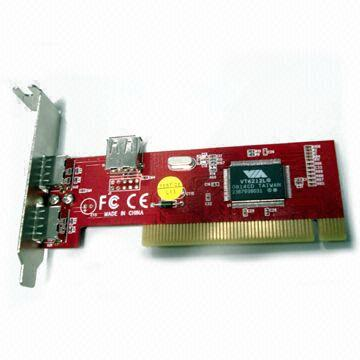
\includegraphics[height=70pt]{pictures/pci_card.jpg}}
                \fbox{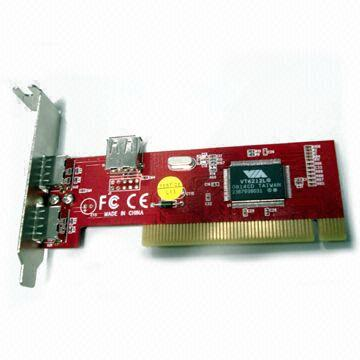
\includegraphics[scale=0.2]{pictures/pci_card.jpg}}
            \end{center}
            \scriptsize{
                Description du périphérique :
                \begin{itemize}
                    \item Registres ;
                    \item Algorithmes.
                \end{itemize}
            }
        }
    \end{column}

    % Center column for Middle-end (\rtx\ Maintainer)
    \begin{column}[c,T]{115pt}
        \uncover<3-> {
            \begin{center} \large{\itshape{Développeur \rtx}} \end{center}
            \scriptsize{
                Identification des sémantiques communes à tous les systèmes
                d'exploitation afin d'en tirer un modèle générique.
            }
        }
    \end{column}
    
    % Right column for Back-end (OS developer)
    \begin{column}[r,T]{115pt}
        \uncover<4-> {
            \begin{center} \large{\itshape{Développeur Système}} \end{center}
            \scriptsize{
                Code spécifique aux systèmes d'exploitation. Requiert des
                connaissances systèmes poussées.
            }
        }
    \end{column}

    \transdissolve<2>
    \transdissolve<3>
    \transdissolve<4>
\end{columns}
\end{frame}

\subsection{Le rôle de chaque partie du DSL}
\begin{frame}
\frametitle{Un DSL en trois parties}
\begin{columns}[c]
    
    \begin{column}[l,T]{115pt}
        \begin{center} \large{\itshape{Front-End}} \end{center}
        \scriptsize{
            \begin{center} Fichier \texttt{.rtx} \end{center}
            Il contient une description :
            \begin{itemize}
                \item Physique du matériel (registres) ;
                \item Algorithmique du pilote ;
                \item Une configuration (sous-systèmes à utiliser, informations
                                         spécifiques à chaque système
                                         d'exploitation...).
            \end{itemize}
        }
    \end{column}
    
    \begin{column}[c,T]{115pt}
        \begin{center} \large{\itshape{Middle-End}} \end{center}
        \scriptsize{
            \begin{center} Fichier \texttt{.rti} \end{center}
            Il contient des interfaces de sous-systèmes décrivant :
            \begin{itemize}
                \item Des Types ;
                \item Des Séquences ;
                \item Des variables de configuration.
            \end{itemize}
        }
    \end{column}
    
    \begin{column}[r,T]{115pt}
        \begin{center} \large{\itshape{Back-End}} \end{center}
        \scriptsize{
            \begin{center} Fichier \texttt{.blt} \end{center}
            Il permet d'implémenter le code système-spécifique correspondant
            aux interfaces associées. On y retrouvera :
            \begin{itemize}
                \item Des templates de type ;
                \item Des templates de séquence.
            \end{itemize}
            Chaque morceau de code instrumenté qui s'y trouve est appelé
            ``placeHolder''.
        }
    \end{column}

\end{columns}
\transdissolve<1>
\end{frame}

\subsection{Illustration de la syntaxe}
\begin{frame}
\frametitle{Introduction à la programmation aspectuelle}
\end{frame}


\begin{frame}
\frametitle{Syntaxe d'une interface}
\only<1> {
    Cinq types d'éléments à implémenter :
    \begin{itemize}
        \item Types ;
        \item Séquences ;
        \item Variables ;
        \item Pointcuts ;
        \item Chunks.
    \end{itemize}
}
\only<2> {
    Quatre mots clefs pour identifier qui implémente quoi.
    Ces mot clefs s'appliquent aux séquences, types et variables.
    \begin{itemize}
        \item provided ;
        \item required ;
        \item optional ;
        \item auto.
    \end{itemize}
}
\only<3> {
    Deux mots clefs pour identifier qui implémente quoi pour la partie
    aspectuelle de \rtx.
    \begin{itemize}
        \item provided ;
        \item use.
    \end{itemize}
}
\only<4> {
    Tableau de croisement des mot clefs avec leur implication pour le
    Front-End et le Back-End :
    \center {
    \begin{tabular}{|l|c|c|c|}
        \hline
             & Front  & Back & Generation  \\
        \hline
        \textcolor{tblB}{auto}     & \textcolor{tblR}{Non}
            & \textcolor{tblG}{Oui} & \textcolor{tblG}{Oui} \\
        \hline
        \textcolor{tblB}{provided} & \textcolor{tblR}{Non}
            & \textcolor{tblG}{Oui} & Si utilisé  \\
        \hline
        \textcolor{tblB}{required} & \textcolor{tblG}{Oui}
            & \textcolor{tblG}{Oui} & \textcolor{tblG}{Oui} \\
        \hline
        \textcolor{tblB}{optional} & Possible
            & Oui si redéfini & Si utilisé  \\
        \hline
    \end{tabular}
    }
}
\transdissolve<2>[duration=0.4]
\transdissolve<3>[duration=0.2]

%\transwipe<2>[direction=90]
\end{frame}


\begin{frame}[containsverbatim]
\frametitle{Exemple d'interface}
\lstset{
    basicstyle=\color{black}\tiny\ttfamily,
    numberstyle=\tiny\ttfamily
}
\begin{lstlisting}
/*
 * This interface describes the basic needs for
 * any loadable kernel module
 */
   interface LKM
   {
       builtin  type       Device;

       provided pointcut   include_dependencies;
       provided pointcut   global_data_declaration;
       provided pointcut   code_declaration;
       provided pointcut   lkm_base_code_definition;

       provided sequence   load()
       {
           provided pointcut   lkm_init_fptrs;
           use      pointcut   lkm_base_code_definition;
       }

       provided sequence   unload()
       {
           provided pointcut   unload_setup;
           use      pointcut   lkm_base_code_definition;
       }
   }
\end{lstlisting}
\end{frame}

\begin{frame}
\frametitle{Exemple de template}
%begin{lstlisting}
%*
%* This is a comment test
%*/
%end{lstlisting}
\end{frame}

\begin{frame}
\frametitle{Exemple d'implémentation de pilote}
%begin{lstlisting}
%*
%* This is a comment test
%*/
%end{lstlisting}
\end{frame}




\section{Un compilateur hors normes}

\subsection{Compilateur classique}
\begin{frame}
\frametitle{Méthode de traduction classique}
\begin{enumerate}[<+->]
    \item Analyse du langage source (construction d'un AST) ;
    \item Manipulation de l'AST pour extraire des schémas d'execution connus ;
    \item Altération optionnelles de l'AST (optimisations, etc...) ;
    \item Traduction du langage source en langage destination selon des
            modèles fixés.
\end{enumerate}
\end{frame}

\subsection{Compilateur \rtx}
\begin{frame}
\frametitle{Méthode de traduction de \rtx}
\begin{enumerate}[<+->]
    \item Analyse du langage source (construction d'un AST) ;
    \item Vérification des types à l'aide des interfaces du Middle-End ;
    \item Sélection des templates utilisés par le Front-End (appels,
            redéfinitions, etc...) ;
    \item Début de la génération par le code global de l'interface le
            plus haut-niveau (LKM) ;
    \item Résolution des templates/chunks/pointcuts chargés à l'aide des
            données décrites dans le Front-End de manière récursive ;
    \item Assemblage des ASTs en remontant la résolution ;
\end{enumerate}
\end{frame}



\subsection{Les implications du DSL}
\begin{frame}
\frametitle{Les composants}
\begin{itemize}[<+->]
    \item CNorm ;
    \item rtxParse : ensemble des règles définissant la syntaxe du DSL ;
    \item RtxNode : normalisation des éléments constituant l'AST ;
    \item rtxLink : gestion d'un cache des interfaces et templates enregistrés ;
    \item rtxTpl : résolution récursive du code instrumenté des templates ;
    \item Tool : outil de génération de fichiers annexes (\texttt{.inf},
                 \texttt{Makefiles}, etc...).
\end{itemize}
\end{frame}


\subsection{Les différents processus de compilation}
\begin{frame}
\frametitle{Compilation du Middle-End}
\begin{itemize}[<+->]
    \item Analyse syntaxique du code ;
    \item Validation des dépendances ;
    \item Validation de l'interface elle-même.
\end{itemize}
\end{frame}

\begin{frame}
\frametitle{Compilation du Back-End}
\begin{itemize}[<+->]
    \item Analyse syntaxique du code C instrumenté ;
    \item Validation des prototypes de templates ;
    \item Validation de la présence des éléments de programmation aspectuelle
            requis par l'interface ;
    \item Extraction des PlaceHolders.
\end{itemize}
\end{frame}

\begin{frame}
\frametitle{Compilation du Front-End}
\begin{itemize}[<+->]
    \item Analyse syntaxique du code ;
    \item Validation des dépendances ;
    \item Validation de l'interface elle-même.
\end{itemize}
\end{frame}




\end{document}
